% !TEX root=/home/tavant/these/manuscript/src/manuscript.tex

\section{Modeling the dielectric layer }
  \label{sec-diel_layer}
  
  The first effect of the wall material studied is adding a layer of dielectric material with its own permittivity, as introduced in \Cref{sec-diel}.
  The simulation parameters are the same as in the canonical case, presented in \cref{sec-canonical}, but the plasma is separated from the ground wall by a dielectric layer of 3~mm.
  Hence, the distance between the grounded electrodes is $2.6\,\centi\meter$.
  The relative permittivity of the dielectric is $\epsr=25$.
  %% SEE runs 250et 257 ?? Ly=1cm, Diel avec et sans SEE
  
  \Cref{fig-diel_radial_Er} shows the radial profile of the radial electric field $E_R$ at $t=10\,\micro\second$ averaged in the azimuthal direction.
  The plasma domain starts at $r=0$ and ends at $r=2\,\centi\meter$.
  We note the jump in the value of the electric field at the plasma-wall transition.
  This jump is due to the surface charge.
  We can also notice that in the dielectric layer, in $r < 0$ and $r > 2\,\centi\meter$, the radial electric field is close to zero, compared to the value in the sheath.
  
  \begin{figure}[hbt]
    \centering
    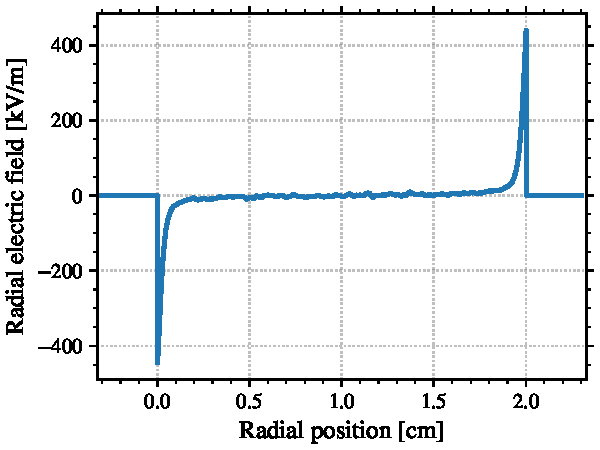
\includegraphics[width=\defaultwidth]{diel_average_radial_electric_field}
    \caption{Radial profile of the radial electric field $E_R$ averaged in the azimuthal direction at $t=10\,\micro\second$. The plasma domain starts at $r=0$ and ends at $r=2\,\centi\meter$. The dielectric length is $L_{\\rm Diel} = 3\,\milli\meter$.  }
    \label{fig-diel_radial_Er}
  \end{figure}
  
  The next sections investigate the impact of the dielectric layer on the plasma characteristics, and highlight the plasma-wall interaction.
  
  \subsection{Effect of the dielectric layer} \label{subsec-effect_mob}
    
  
  The simulation results are qualitatively the same as in the case without the dielectric layer.
  As an example, \Cref{fig-mod_diel_comp} shows the temporal evolution of the axial electron mobility with and without the dielectric layer.
  We see that the results for the electron temperature and mobility are similar.
  The low amplitude oscillation of the case with the dielectric decreases slightly slower.
  
  \begin{figure}[hbt]
    \centering
    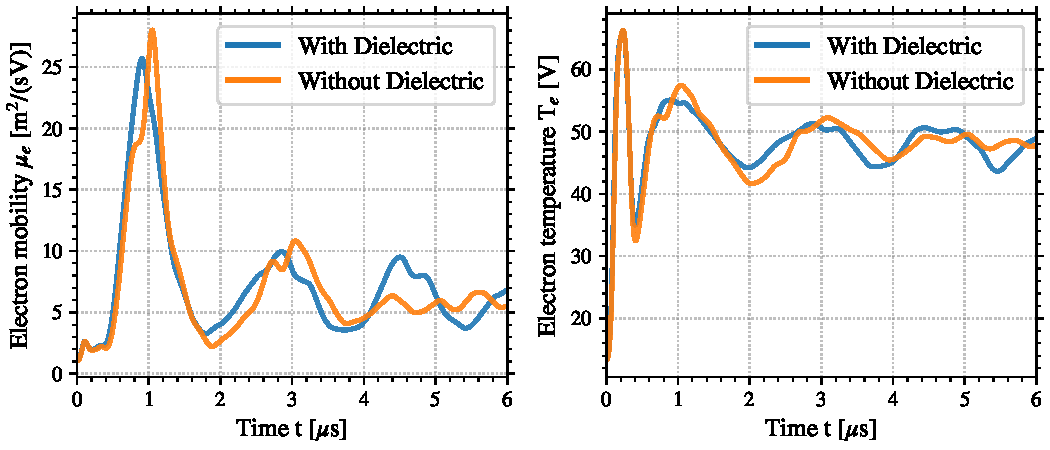
\includegraphics[width=\textwidth]{Dielectric_noSEE_temporal.pdf}
    \caption{Temporal evolution of the axial electron mobility (left), and the electron temperature (right) with and without the dielectric layer modeled.}
    \label{fig-mod_diel_comp}
  \end{figure}

  
  \subsection{Near-wall and in-wall parameters} \label{subsec-nearwall}
    In this section, we focus on the surface charge and the near-wall electric field.
    \Cref{fig-sigma_time} shows the temporal evolution of the surface charge at one point of the wall.
    The position has been chosen to be the center ($L_{\theta} = 0.25$~cm) of the lower wall, but the observations are similar at other positions.
     
    \begin{figure}[!hbt]
      \centering
      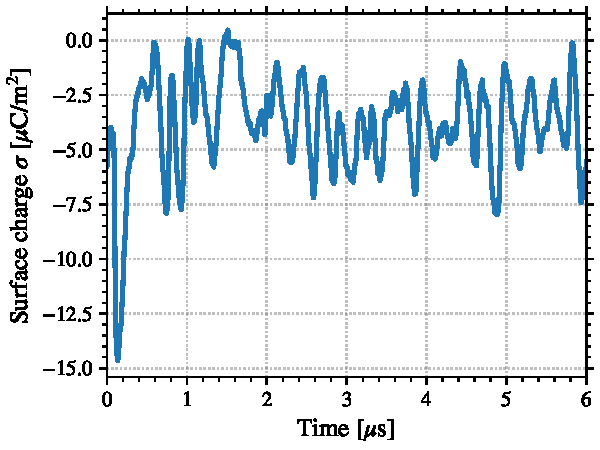
\includegraphics[width=\defaultwidth]{temporal_sigma}
      \caption{Temporal evolution of the surface charge $\sigma$ at one position of the lower dielectric wall}
      \label{fig-sigma_time}
    \end{figure}

    We can see in \cref{fig-sigma_time} that the value of the surface charge start by decreasing significantly (increasing in absolute value), due to the hot electrons that reach quickly the walls.
    Then, $\sigma$ grows and oscillates around a mean value close to $-3.5 \,\micro\coulomb/\square\meter$ and with an amplitude of approximately $1.2 \,\micro\coulomb/\square\meter$.
    
    \cref{fig-indiel} shows the azimuthal evolution of the radial electric field inside the dielectric layer.
    The electric field is given at three different positions ($r=-0.2, -0.9,$ and $-1.8\,\milli\meter$ away from the plasma-wall interface) to highlight its evolution.
    We can see that, even though there is no charge in the dielectric, the amplitude of the electric field decreases when going further away from the plasma.
    This is due to the \ac{2D} Poisson equation, which smooth-out the inhomogeneity.
     
    \begin{figure}[!hbt]
      \centering
      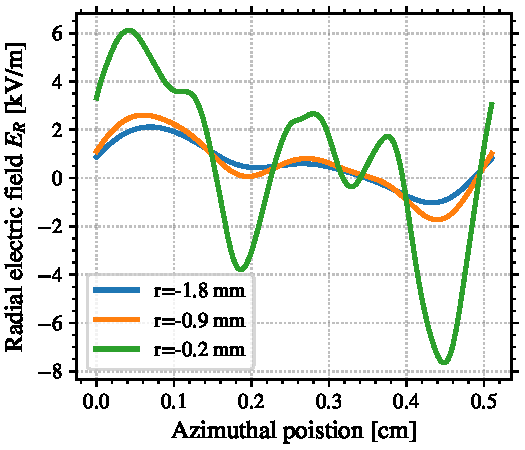
\includegraphics[width=\defaultwidth]{Radial_electric_feld_in_diel.pdf}
      \caption{Azimuthal evolution of the radial electric field inside of the dielectric layer at three different positions; the reference $r=0$ is the plasma-wall interface, the grounded electrode is located at $r=-3\,\milli\meter$.}
      \label{fig-indiel}
    \end{figure}

    
  \subsection{Dielectric model comparison} \label{subsec-modelcomp}

  
  As introduced in \cref{sec-diel}, a simplified approach to model the effect of the surface charges on the plasma is to use a Neumann boundary condition \citep{taccogna2019}
  \begin{equation} \label{eq-neuman}
    E_r = \frac{\sigma}{\epsilon_0}.
  \end{equation}
  \Cref{eq-neuman} uses two approximations\string:
  \begin{itemize}
    \item one dimensional
    \item No electric field in the dielectric
  \end{itemize}
  We have already seen in \cref{fig-indiel} that the electric field in the dielectric is not zero, but instead it oscillates in respect to the azimuthal instability present in the plasma.  
  \Cref{fig-spacial_comparaison} shows the radial electric field at the wall and compares it to what is obtained by \cref{eq-neuman}.
  We can see that the two values are of the same order of magnitude, close to $-500$~kV/m.
  However, the two values are not equal, as they oscillate around their mean value.
  We can see that the surface charge oscillates more than the actual electric field obtained by solving the Poisson equation.

\begin{figure}[!hbt]
  \centering
  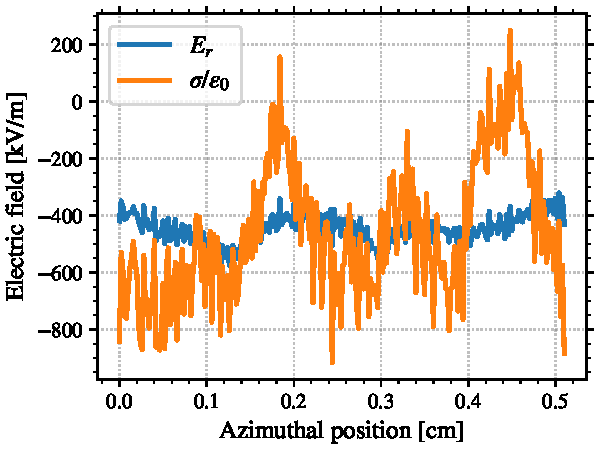
\includegraphics[width=\defaultwidth]{Radila_electric_field.pdf}
  \caption{Azimuthal evolution of the radial electric field at the plasma-wall interface and the electric field that would result from surface charge according to \cref{eq-neuman}.}
  \label{fig-spacial_comparaison}
\end{figure}
\renewcommand\subfigurewidth{0.45\textwidth}

  As a conclusion, we have observed that the dielectric layer does not change the simulation results much, but it can modify the surface processes.
  The model used here for the dielectric layer does not modify the performance of the simulation, while allowing to take into account the \ac{2D} effects.
  In this section, no secondary electron emission has been taken into account.
  In \cref{sec-fulldiel}, we will discuss the influence of using the simplified \cref{eq-neuman} in the case where secondary electron emission is important.

  